\documentclass{article}
\usepackage[left=2cm, right=2cm, top=2cm, bottom=2cm]{geometry}
\usepackage{graphicx} 
\usepackage{url}
\usepackage[utf8]{inputenc}
\usepackage{parskip} 
\setlength{\parskip}{0.5 cm}
\graphicspath{{Imagenes/}}

\title{\vspace{-1.5cm} Curriculum Vitae \\ \Huge{Cristobal Cortés Gómez} \\ \large{Software Developer \& Inventor Mathematician} \\ \normalsize{Proudly Tapatío} \\ 
\vspace{0.3cm}
\normalsize{
legocris@hotmail.com \ $|$ \ +52 33 1115 0013 \\
GitHub: \url{https://github.com/legocris} \ $|$ \ LinkedIn: \url{www.linkedin.com/in/cristobal-cortes-gomez}
}
\vspace{-1cm}}
\author{}
\date{}

\begin{document}

\maketitle

\section*{Professional Profile}
Mathematician with a strong background in abstract algebra and theoretical computer science, complemented by extensive experience as a cross-platform software developer and indie game developer. Specialized in the TypeScript/JavaScript ecosystem for web development, Python for numerical methods and AI, and C/C++ for low-level tools. Experienced in managing complex workflows in Linux environments, utilizing highly customized terminal editors (Emacs, Vim), and solving software architecture challenges, as well as hardware engineering and automation projects.

\section*{Technical Skills}
\textbf{Languages:} TypeScript, JavaScript, C, C++, C\#, Java, Python, Fortran, R, Pascal, Node.js, HTML, LUA, CSS, Less, GML, GLSL, HLSL, CUDA. \\
\textbf{Frameworks \& Libraries:} React, Redux Toolkit, Three.js, Pixi.js, Sklearn, PyTorch. \\
\textbf{Tools \& Engines:} GameMaker Studio, Unity 3D, Processing, Blender. \\
\textbf{Systems \& Workflow:} Linux environments (shell scripting), Git, Emacs, Vim. \\
\textbf{Hardware \& Electronics:} Microcontrollers (ESP8266, Arduino IoT), Siemens PLC, PCB design, circuit diagnostics, and retrofitting vintage devices.

\section*{Languages}
\textbf{Spanish:} Native \\
\textbf{English:} Advanced (Fluent and technical communication with international clients).

\section*{Education}

\textbf{2017-2025}: Bachelor's Degree in Mathematics at Universidad de Guadalajara (CUCEI).

Final Project: Convergence analysis of shallow vs. deep Neural Networks using the perceptron for classification problems.\\
Link: \url{https://drive.google.com/file/d/1y_D-IL4z9spmbDCHWOvdoEBr8vfhC2Ic/view?usp=sharing}\\
Link: \url{https://github.com/legocris/Archivos-Proyecto-Analisis-de-Convergencia-RN}

\section*{Work Experience}

\textbf{2025-2026}: Freelance Software Developer for a 2D action game designed to teach programming. Its key feature allows players to program the character's superpowers using JavaScript.

Client: Gnarled Helix LLC \\
Links: \url{https://open-sourcerer.com/} \\
Images:
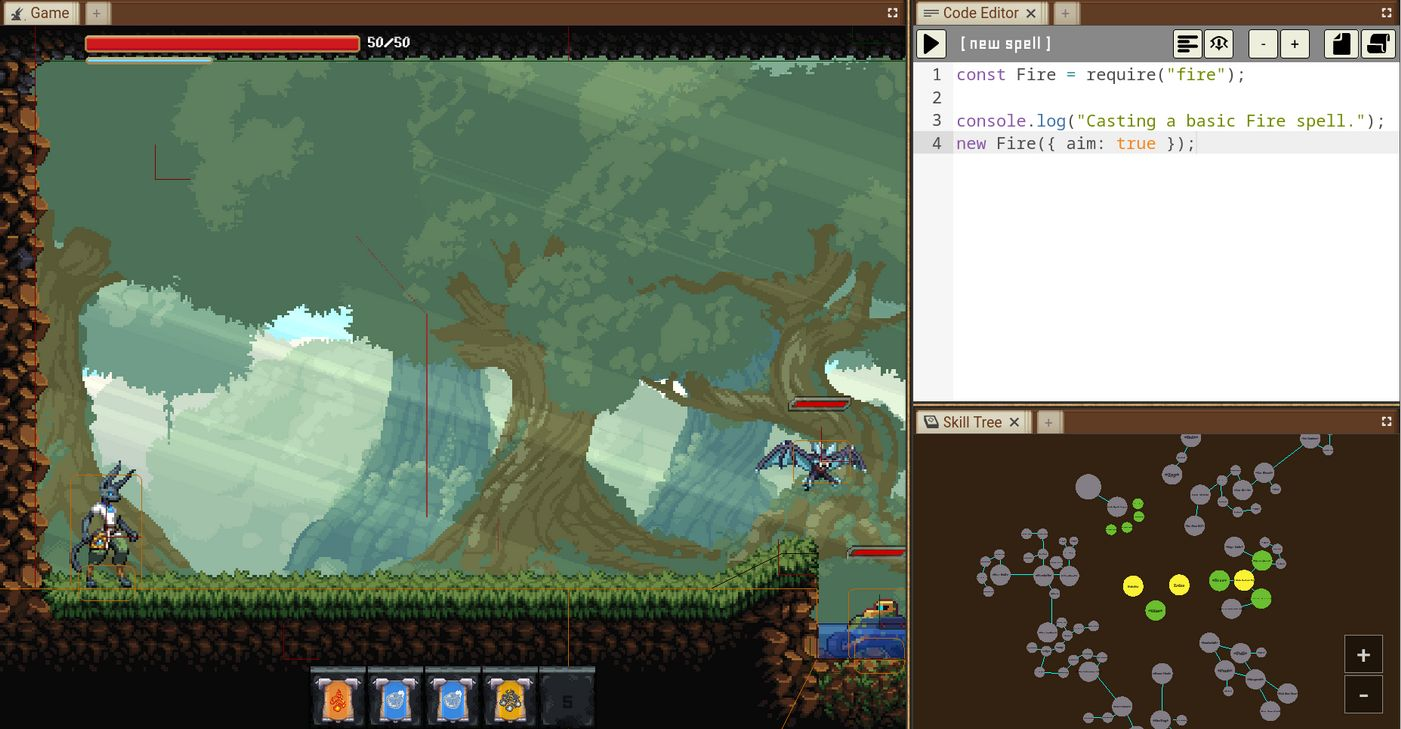
\includegraphics[width=0.45\textwidth, height=3.5cm, keepaspectratio]{Gnarled Elix.jpg}

\textbf{2024-2025}: Designer and Lead Software Developer for the video game adaptation of the board game "Camino a Xibalbá PITZ".

Client: Jalapeño Labs. \\
Links: \url{https://jalapenolab.mx/pages/pitz} \\
Technologies used: GameMaker:Studio, JavaScript, Firebase. \\
Images:
    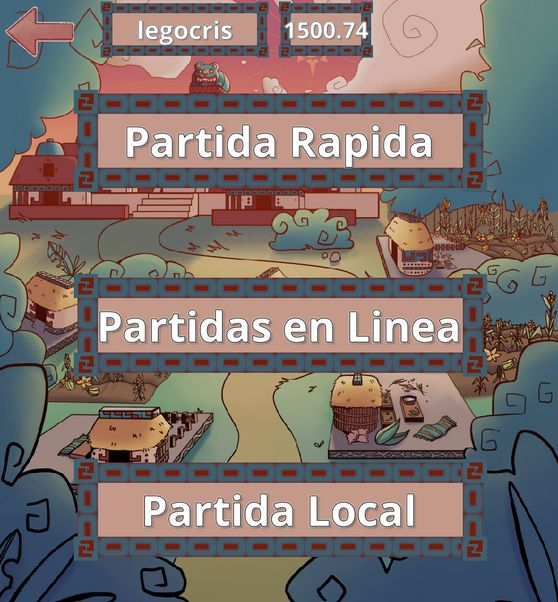
\includegraphics[width=0.35\textwidth, height=3cm, keepaspectratio]{Jalapeño0.jpg}\hspace{0.5cm}%
    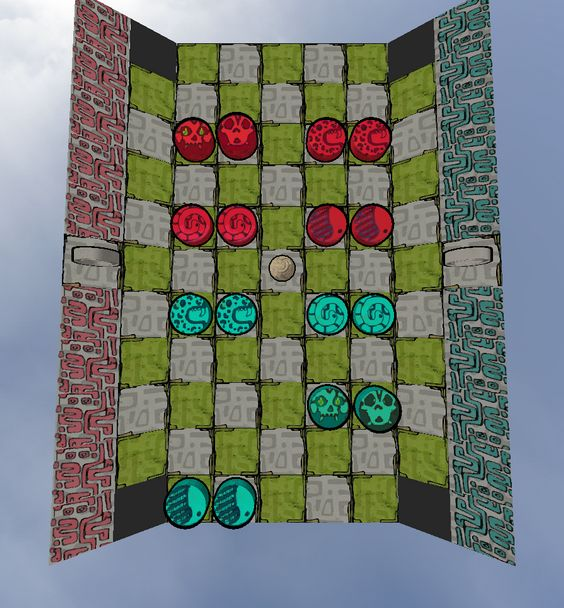
\includegraphics[width=0.35\textwidth, height=3cm, keepaspectratio]{Jalapeño.jpg}

\textbf{2023-2025}: Automated Greenhouse for edible mushroom cultivation. Construction of an automated greenhouse featuring humidity and temperature controls, including the complete electrical installation.

Technologies used: ESP8266 Microcontroller, Arduino IoT, PCB Design. \\
Video: \url{https://drive.google.com/file/d/1VXNXsHJxxcXPUsZ7u1oSj_WJdibgUq9U/view?usp=drive_link} \\
Images:
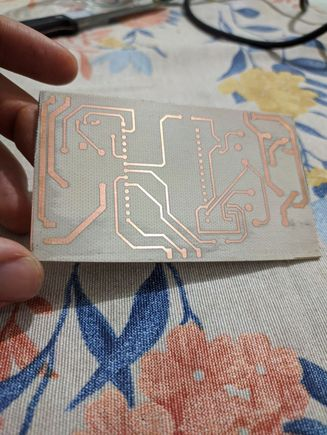
\includegraphics[width=0.25\textwidth, height=3cm, keepaspectratio]{Inti1.jpg}\hspace{0.4cm}%
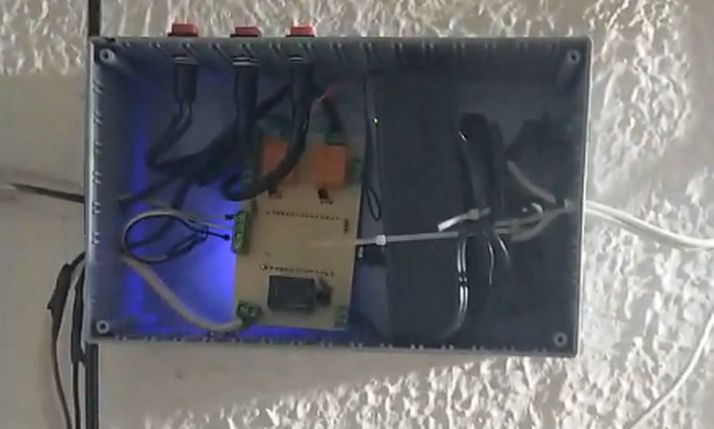
\includegraphics[width=0.25\textwidth, height=3cm, keepaspectratio]{Inti2.jpg}\hspace{0.4cm}%
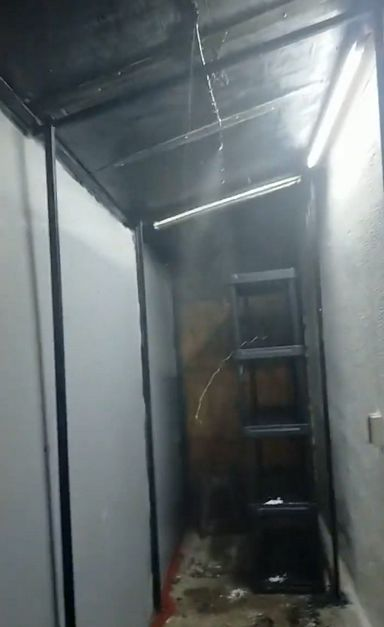
\includegraphics[width=0.25\textwidth, height=3cm, keepaspectratio]{Inti3.jpg}

\textbf{2022-2025}: Mathematics Tutor. Private math tutoring for teenagers and adults.

\textbf{2022}: Robotics Instructor for children (one semester).

Client: American World Languages (AWL Chapultepec) \\
Video: \url{https://drive.google.com/file/d/1jcYXvor1MOY12M_HYyBxCDk3AN8kvsEa/view?usp=sharing} \\
Images:
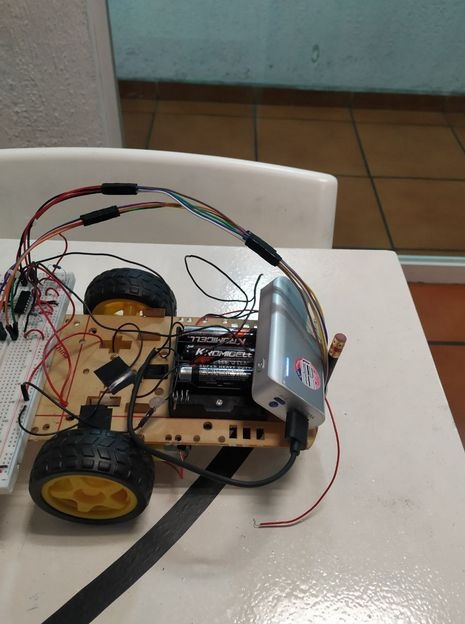
\includegraphics[width=0.45\textwidth, height=3.5cm, keepaspectratio]{AmericanWorldLanguages.jpg}

\textbf{2020-2022}: Artistic Experimentation Work for a social and artistic project on intersexuality. Developed an LED face mask capable of displaying simple custom images, along with a 3D Museum Simulator.

Technologies used: JavaScript, Arduino, ESP8266 Microcontroller, Blender, Unity 3D. \\
Client: Proyecto INTERSEX \\
Links: \url{https://intersex.mx/}

\textbf{2017-2020}: Web Development for SGT Total, a commercial website selling public lighting equipment. Mobile-responsive website built with HTML and CSS. \\
Links: \url{https://sgt-total.com/}

\textbf{2018}: Upwork: Full development of a mini-game simulating a computer desktop environment where clicking a corrupted file requires players to memorize and retype text shown briefly on screen.

Client: Daniel Douglas \\
Images:
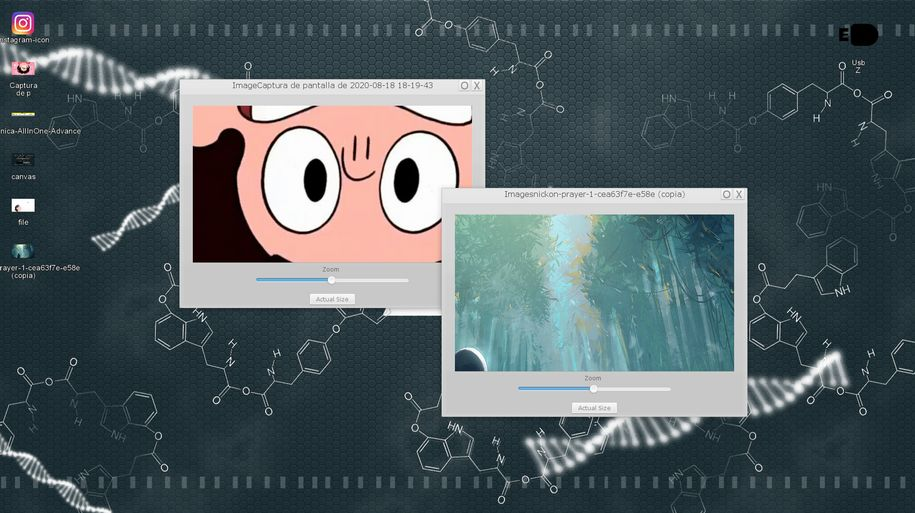
\includegraphics[width=0.35\textwidth, height=3cm, keepaspectratio]{DanielDouglas.jpg}\hspace{0.5cm}%
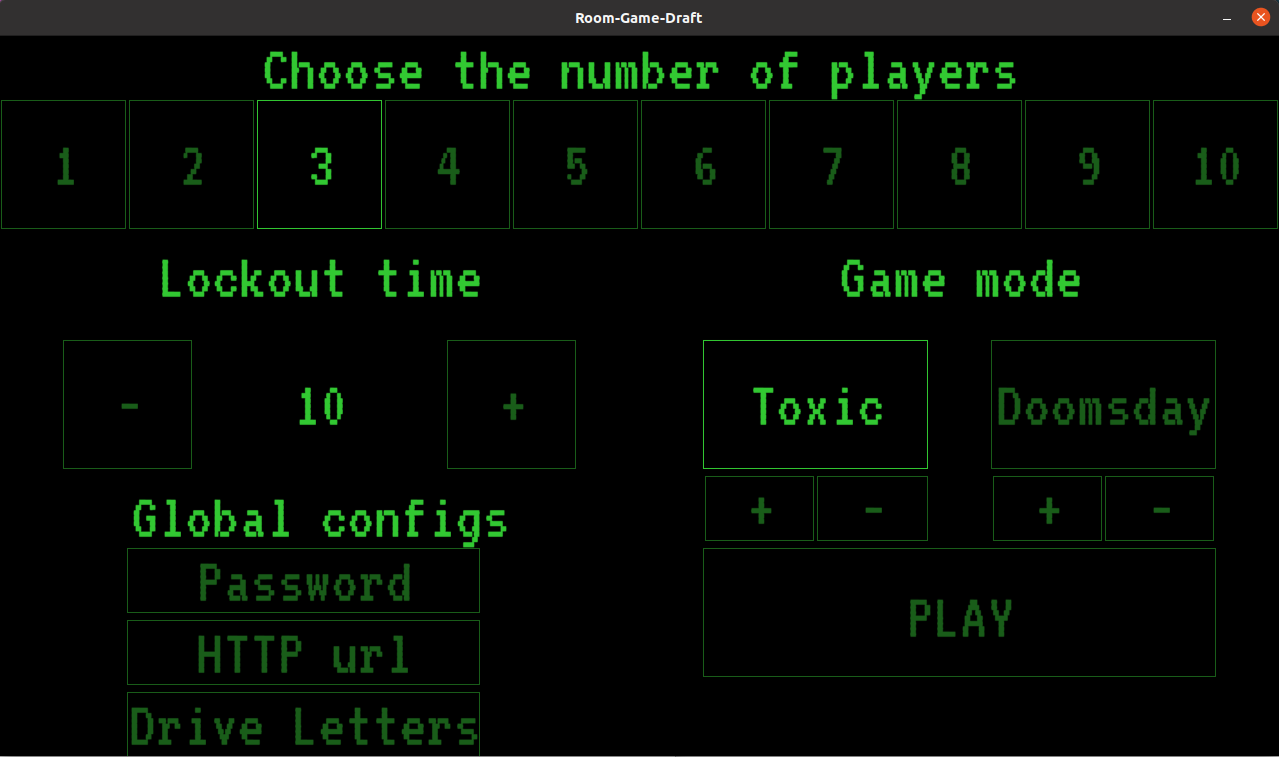
\includegraphics[width=0.35\textwidth, height=3cm, keepaspectratio]{DanielDouglas2.png}

\textbf{2017}: Theater Performance "Habitar". Developed a Kinect application to adjust real-time projections based on physical bar movements.

Client: "Habitar" Theater Show, directed by Velvet Ramírez (Multimedia Team: Selene González and Eduardo Jiménez). \\
Technologies used: Processing, Java, GLSL \\
Links: \url{https://cultura.iteso.mx/web/general/detalle?group_id=5313293}

\textbf{2018}: Upwork: Unity – Shader Conversion and Application. Adapted a GLSL script (shader) to HLSL to implement a spherical/fisheye projection for VR headsets in a medical application.

Technologies used: GLSL, HLSL, Unity3D. \\
Client: Immertec, Jon Clagg \\
Images:
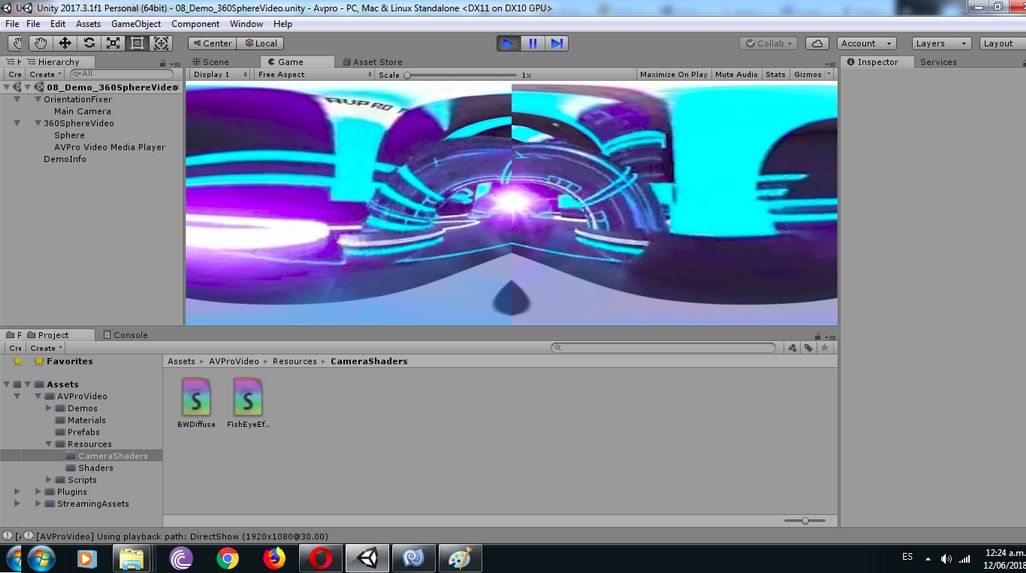
\includegraphics[width=0.45\textwidth, height=3.5cm, keepaspectratio]{Immertec.jpg}

\textbf{2016-2017}: Industrial Design \& Automation. Designed and built a semi-automatic bottle labeling machine. Programmed a PLC for a keg washer/filler system.

Technologies used: Arduino Mega, Siemens PLC, Ladder logic / Flowchart programming. \\
Client: Cervejal \\
Video: \url{https://1drv.ms/v/s!Aslbn4nR5WV3gXMu1zZDiq8jeHbF}


\section*{Completed Independent Projects}

\textbf{2019}: "Me Canso Ganso" Video Game. Co-developer for an arcade mobile game where players control President López Obrador riding a goose, dodging increasingly fast obstacles.

Technologies used: GameMaker:Studio 2, GML language. \\
APK Links (removed from store): \\
\url{https://apkpure.com/de/me-canso-ganso/com.piratagamesparatu.mecansoganso/download/1.0.0} \\
\url{https://drive.google.com/file/d/1a3S5-g950tGvitwL9Aq6CDquU3H9GVtZ/view?usp=sharing}

\textbf{2018}: "Sacrifice Your Brothers" Video Game. Co-developer for a local multiplayer arcade action game where players choose between saving teammates or sacrificing them in an urn to extend their own survival time.

Links: \url{https://axolotlbros.itch.io/sacrifice-your-brothers} \\
Images:
\begin{center}
    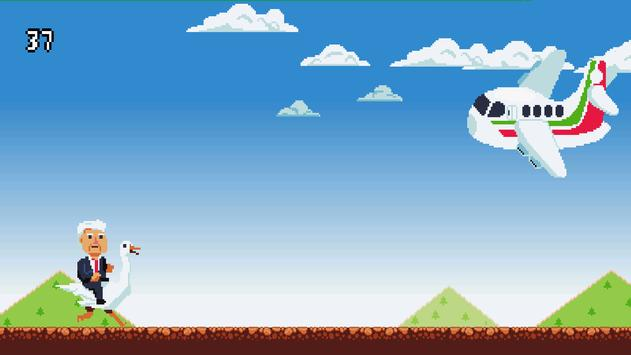
\includegraphics[width=0.25\textwidth, height=3cm, keepaspectratio]{AxolotlBros1.png}\hspace{0.4cm}%
    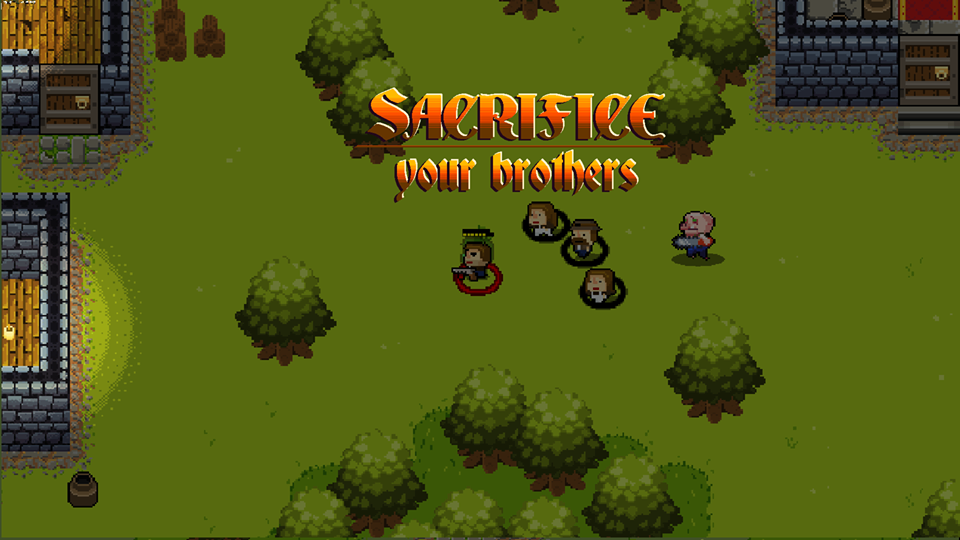
\includegraphics[width=0.25\textwidth, height=3cm, keepaspectratio]{AxolotlBros2.png}\hspace{0.4cm}%
    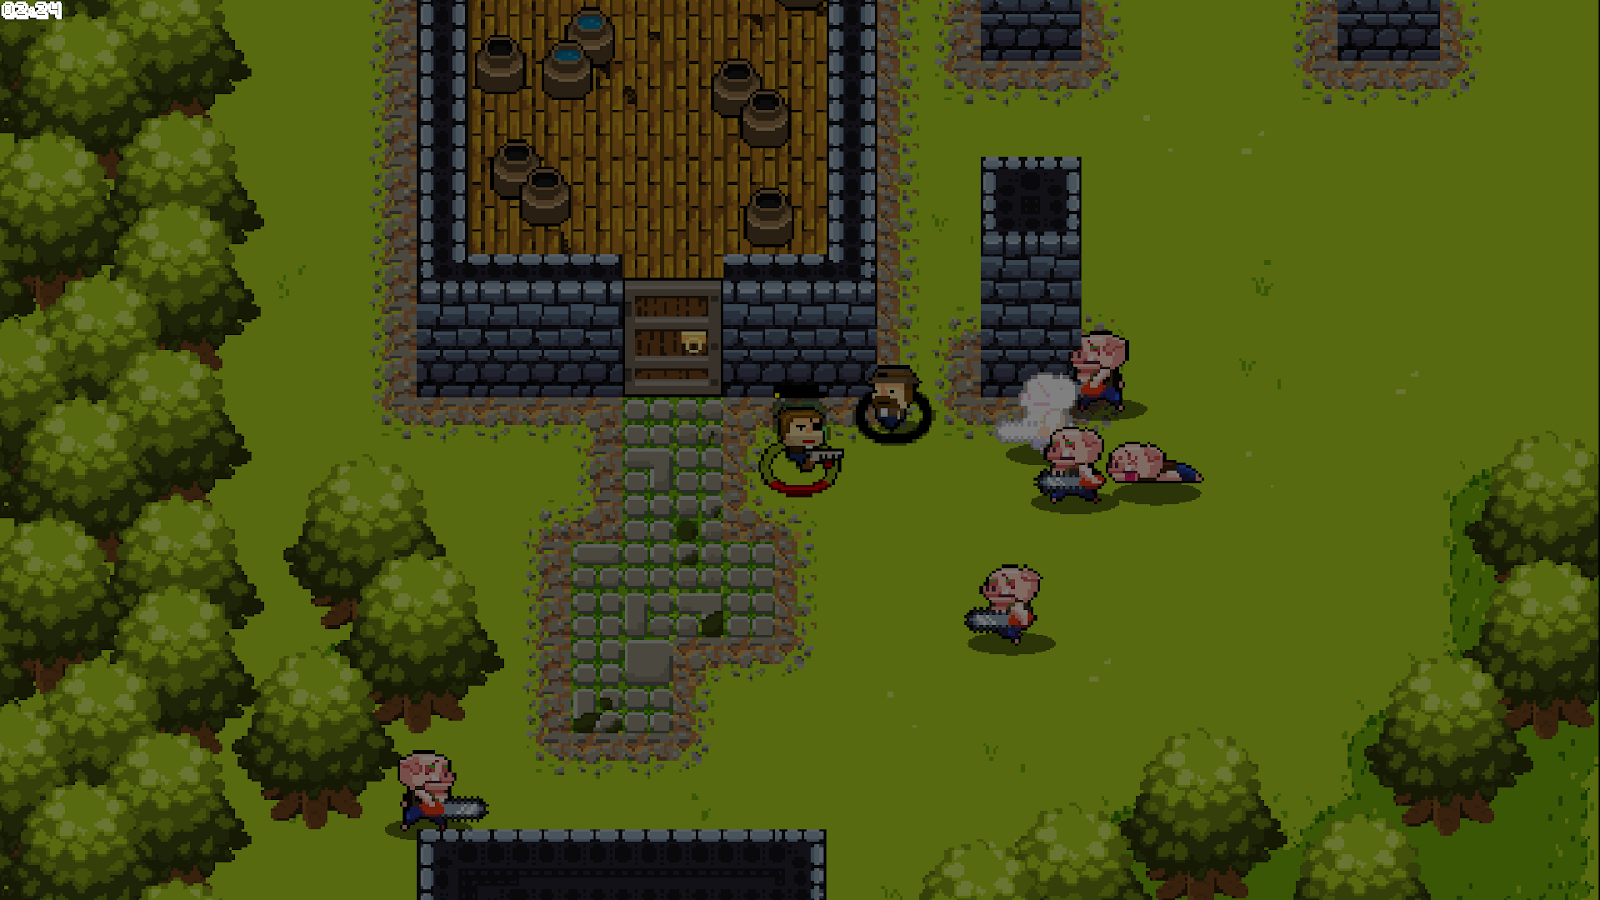
\includegraphics[width=0.25\textwidth, height=3cm, keepaspectratio]{AxolotlBros3.png}
\end{center}

\textbf{2014}: "Sweet Valentine’s Day" Video Game. Lead developer for a mobile arcade game where players play as Cupid, linking couples while shooting arrows to defeat match-ruining enemies.

APK Links (removed from store): \\
\url{https://apkpure.com/sweet-valentine-s-day-free/com.axolotl.svdayfree} \\
\url{https://drive.google.com/file/d/1MA1SfxKcKKX8VI8fpP4RzvQA85vqMPDv/view?usp=sharing}\\
Images:
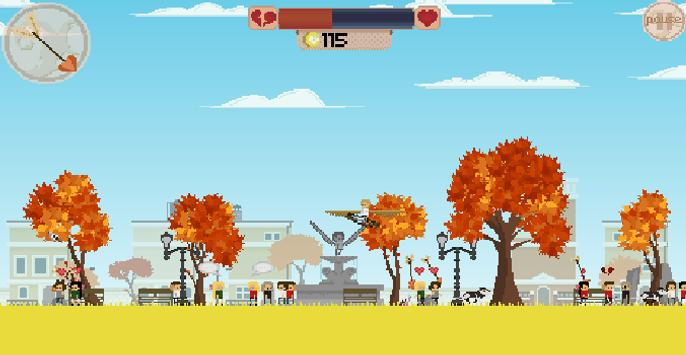
\includegraphics[width=0.35\textwidth, height=3.5cm, keepaspectratio]{AxolotlGames.png}

\textbf{2012}: "Morbus" Video Game. Survival arcade game where players defend against zombie waves, upgrading weapons using earned currency. Awarded a bronze medal at the "Proyecto Multimedia" competition in \textbf{2012}.

Executable Link: \url{https://drive.google.com/file/d/1DNkXIkSf1YP37GFBk0NhI1SNT005FhZE/view?usp=sharing} \\
Images:
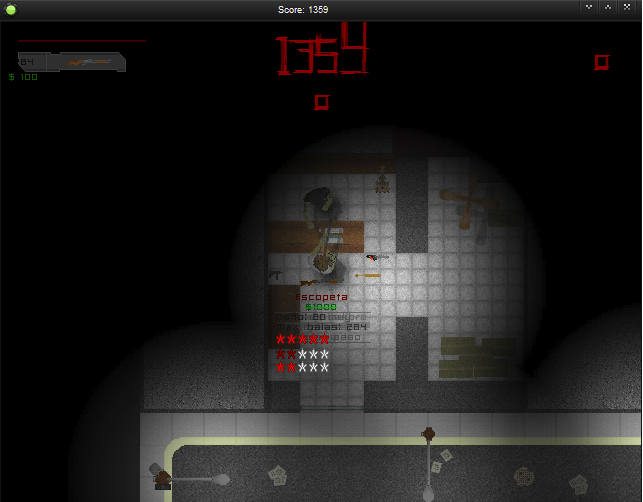
\includegraphics[width=0.45\textwidth, height=3.5cm, keepaspectratio]{ProyectoMultimedia.png}

\section*{Courses \& Academic Updates}
Escuela de Matemáticas de Occidente (EMO 2024) (40 hrs): \\ 
Link: \url{https://www.facebook.com/share/p/194nTvHzMR/} \\
PredGenIA (2023) Deep Learning Methods for Genomic Prediction (20 hrs). \\ Link: \url{https://silo.uy/vufind/Record/REDI_9e7d18e2dc02c81f054dbc56c7acd0d1/Details?sid=7802947} \\
VI Summer School in Mathematics CUCEI (2022 \& 2023) Intensive training (60 hrs): \\
Link: \url{https://www.cucei.udg.mx/carreras/matematicas/es/video/escuela-de-verano-en-matematicas}

\section*{Other Links}
Interview at GAME DEV XPerience \textbf{2018} UNAM: \\
\url{https://www.youtube.com/watch?v=Jzu9Uo8_aTk}

Global Game Jam Projects created in 48hrs (since \textbf{2012}): \\
\url{https://www.youtube.com/watch?v=sKryIP7iI3w} \\
\url{http://2013.globalgamejam.org/2013/sweet-valentines-day} \\
\url{http://globalgamejam.org/2016/games/devils-best-friend}\\
\url{https://v3.globalgamejam.org/2018/games/chromobot-fighters-roboffice-edition}\\
\url{https://v3.globalgamejam.org/2019/games/la-casa-del-roboritmo}\\
\url{https://v3.globalgamejam.org/2020/games/pits-fire-4}\\
\url{https://globalgamejam.org/games/2024/comrade-spatial-baby-9}


Independent project AXOLOTL BROTHERS:
\url{https://www.youtube.com/@axolotlbrothers1253} \\
\url{https://axolotlbros.itch.io/} \\
\url{https://www.facebook.com/AxolotlBros/} \\
\url{https://x.com/axolotlbros?lang=ar-x-fm}

\end{document}